\documentclass[10pt,aspectratio=43]{beamer}

\usepackage{graphicx}
\usepackage{tikz}
\usepackage{xcolor}
\usepackage{caption}
\usepackage{subcaption}
\usepackage{bm}
\usetikzlibrary{calc} 
\usepackage{hyperref}
\hypersetup{
    colorlinks=true,
    linkcolor=blue,
    urlcolor=red
}
\usepackage{fontawesome5}
\usepackage{ulem}
\usepackage[dvipsnames]{xcolor}

\usetheme{MyStyle}   % loads beamerthemeMyStyle.sty
\setlength{\columnsep}{0pt}


%%%%%%%%%%%%%%%%%%%%%%%%%%%%%%%%%%%%%%%%%%
%%%%%%%%%%%%%%%%%%%%%%%%%%%%%%%%%%%%%%%%%%
%%%%%%%%%%%%%%%%%%%%%%%%%%%%%%%%%%%%%%%%%%

\title{Coherent DVCS off $^4\mbox{He}$ with ALERT and CLAS at JLab}
\newcommand{\eventname}{ECT* Workshop}
\author{Felix Touchte Codjo}
\institute{IJCLab}
%\date{\today}
\date{November 10, 2026}


\begin{document}

\begin{frame}[plain] % remove header, footer, barre de navigation
\titlepage
\end{frame}


\begin{frame}{Nuclear GPDs}
    \begin{itemize}
        \item The Generalized Parton Distributions (GPDs) combine the notion of PDFs and FFs, along with their correlations 
            % \begin{itemize}
            %     \item 3D imaging, spin puzzle, distribution of pressure and shear forces
            % \end{itemize}
        \item We can access GPDs off the free proton or off a nucleus
        \item A direct comparison of these distributions can reveal a variety of nuclear effects
            \begin{itemize}
                \item \textit{e.g.} modification of the quark confinement size, short range correlation
            \end{itemize}
        \item This will provide new insights into the understanding of the EMC effect
    \end{itemize}


    \centering
    \vspace{0.3cm}

    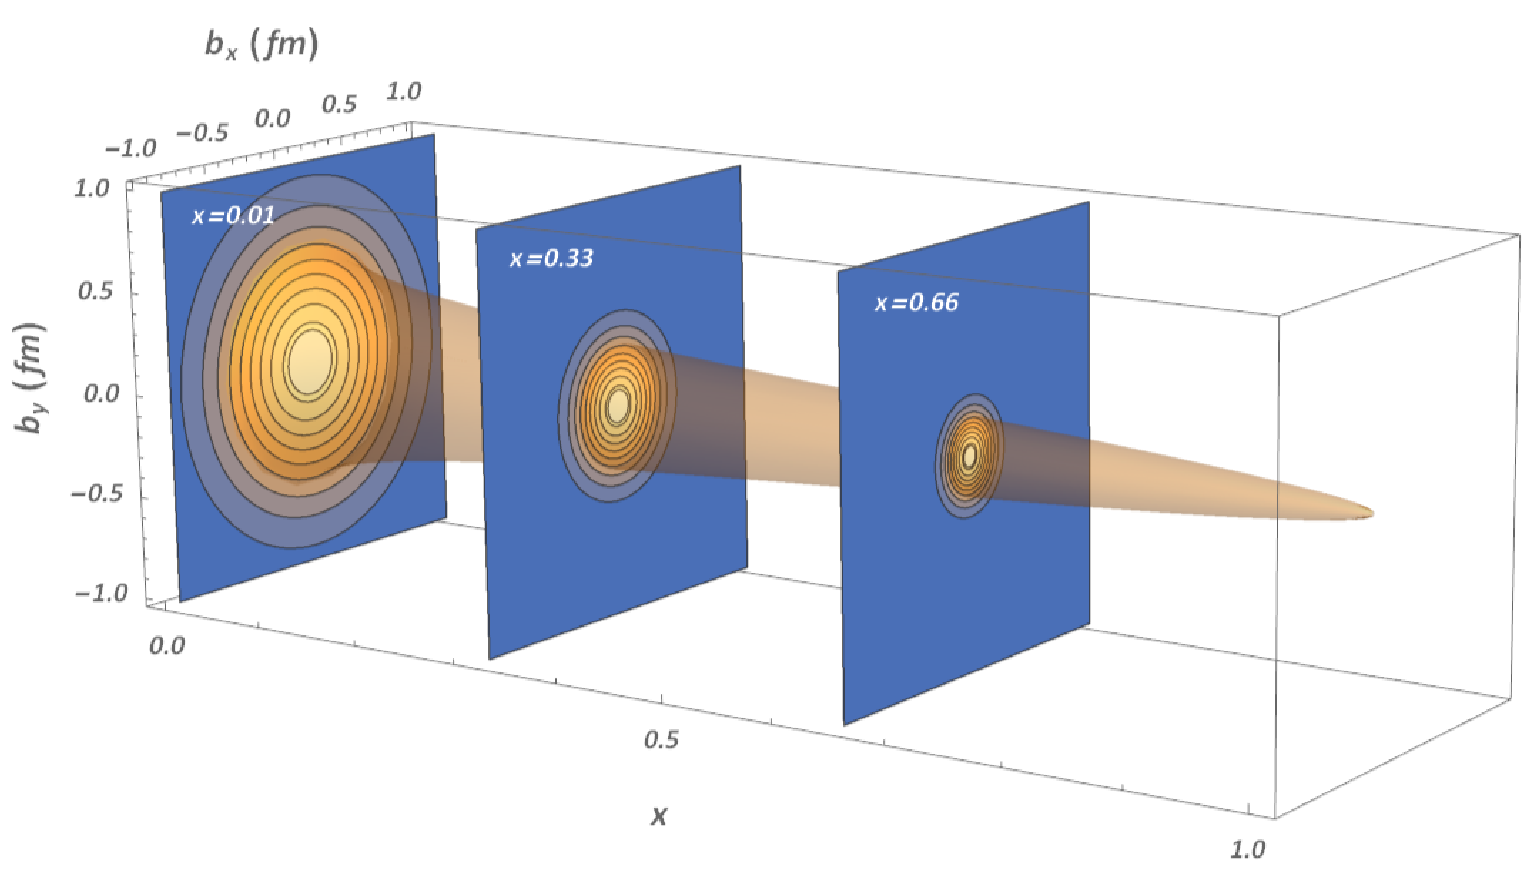
\includegraphics[width=0.45\linewidth]{figures/gpd_3D_imaging.png}
    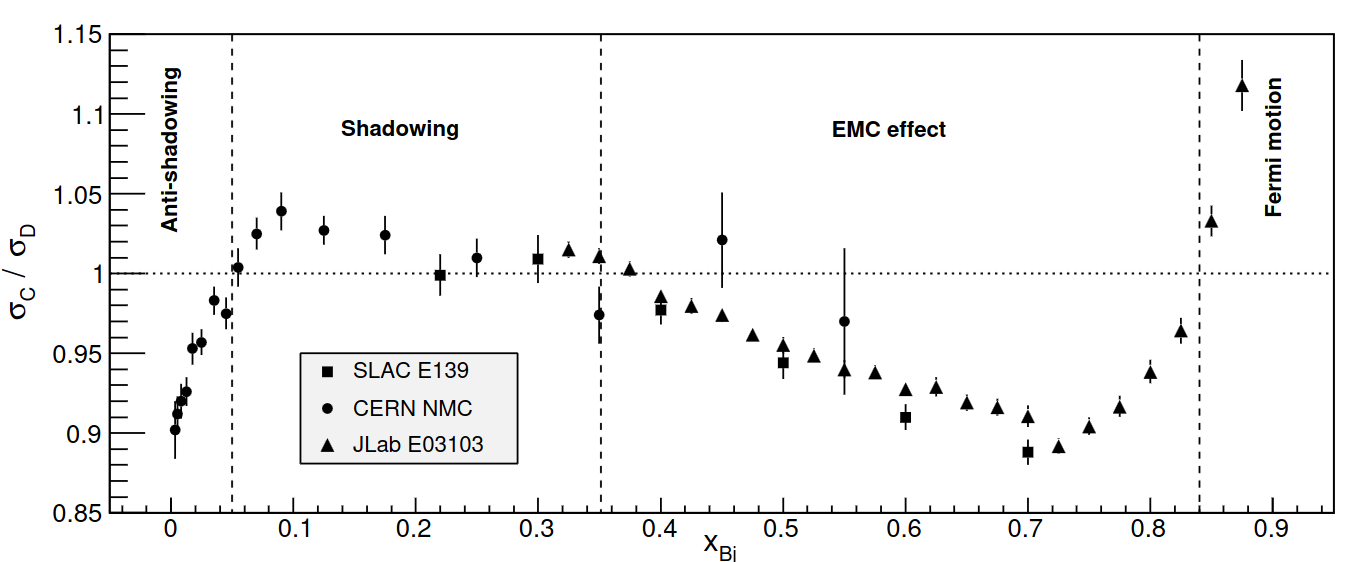
\includegraphics[width=0.45\linewidth]{figures/emc_effect.png}


\end{frame}


\begin{frame}{Nuclear coherent DVCS}

    \begin{minipage}{0.62\linewidth}
        \begin{itemize}
            \item We can access quark GPDs in DVCS
            \item For a nuclear target, the DVCS can be coherent or incoherent
            \item First measurements by HERMES
                \begin{itemize}
                    \item The recoil nuclei were not detected
                    \item $-t$ based threshold to separate the channels
                    \item Measurements affected by large uncertainties
                    \item No nuclear dependence of the BSA found
                \end{itemize}
            \item CLAS eg6 : first coherent DVCS off $^4\mbox{He}$
                \begin{itemize}
                    \item The recoil nucleus was detected
                    \item Coherent and incoherent channels were isolated
                    \item The coherent BSA is twice the one measured on the free proton
                \end{itemize}
        \end{itemize}
    \end{minipage}
    \begin{minipage}{0.35\linewidth}
        
        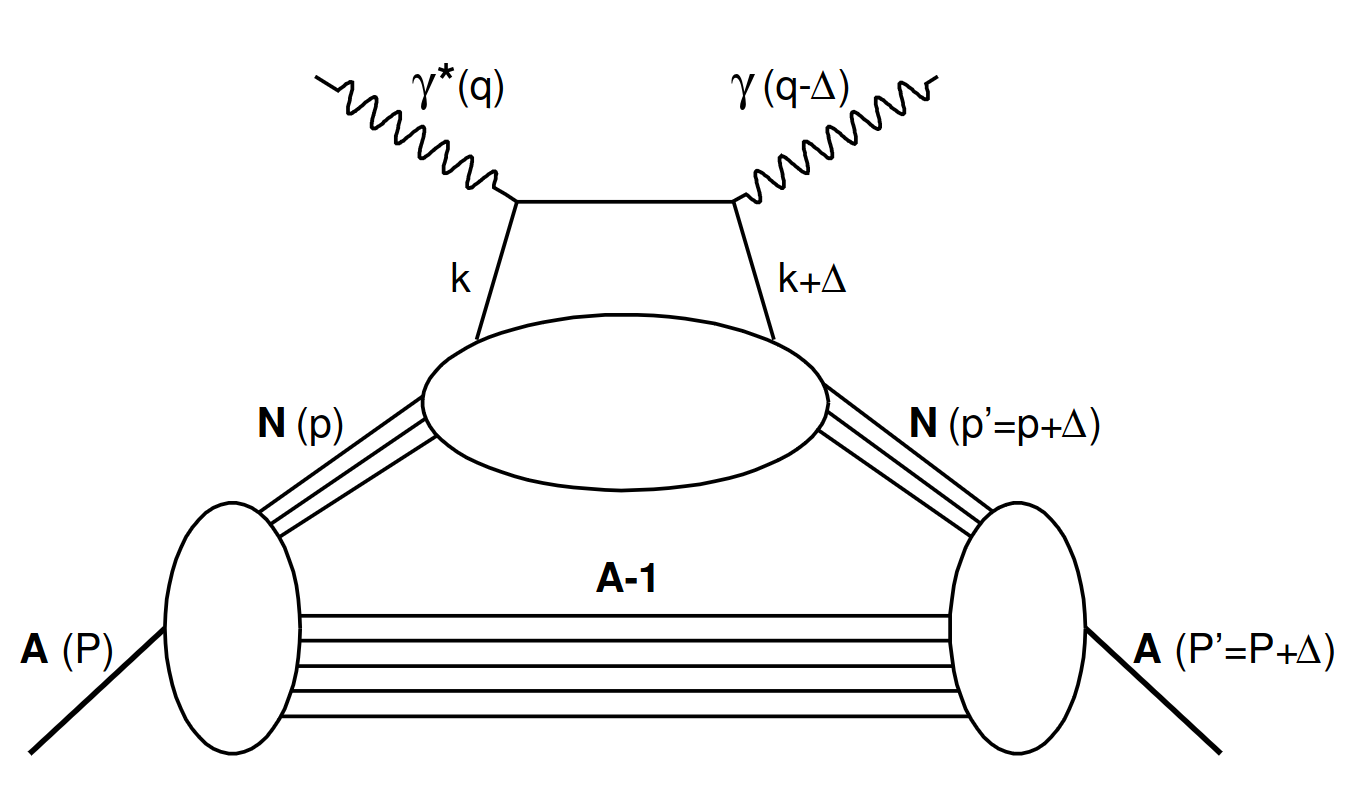
\includegraphics[width=\linewidth]{figures/coherent_dvcs.png}

        \vspace{0.2cm}

        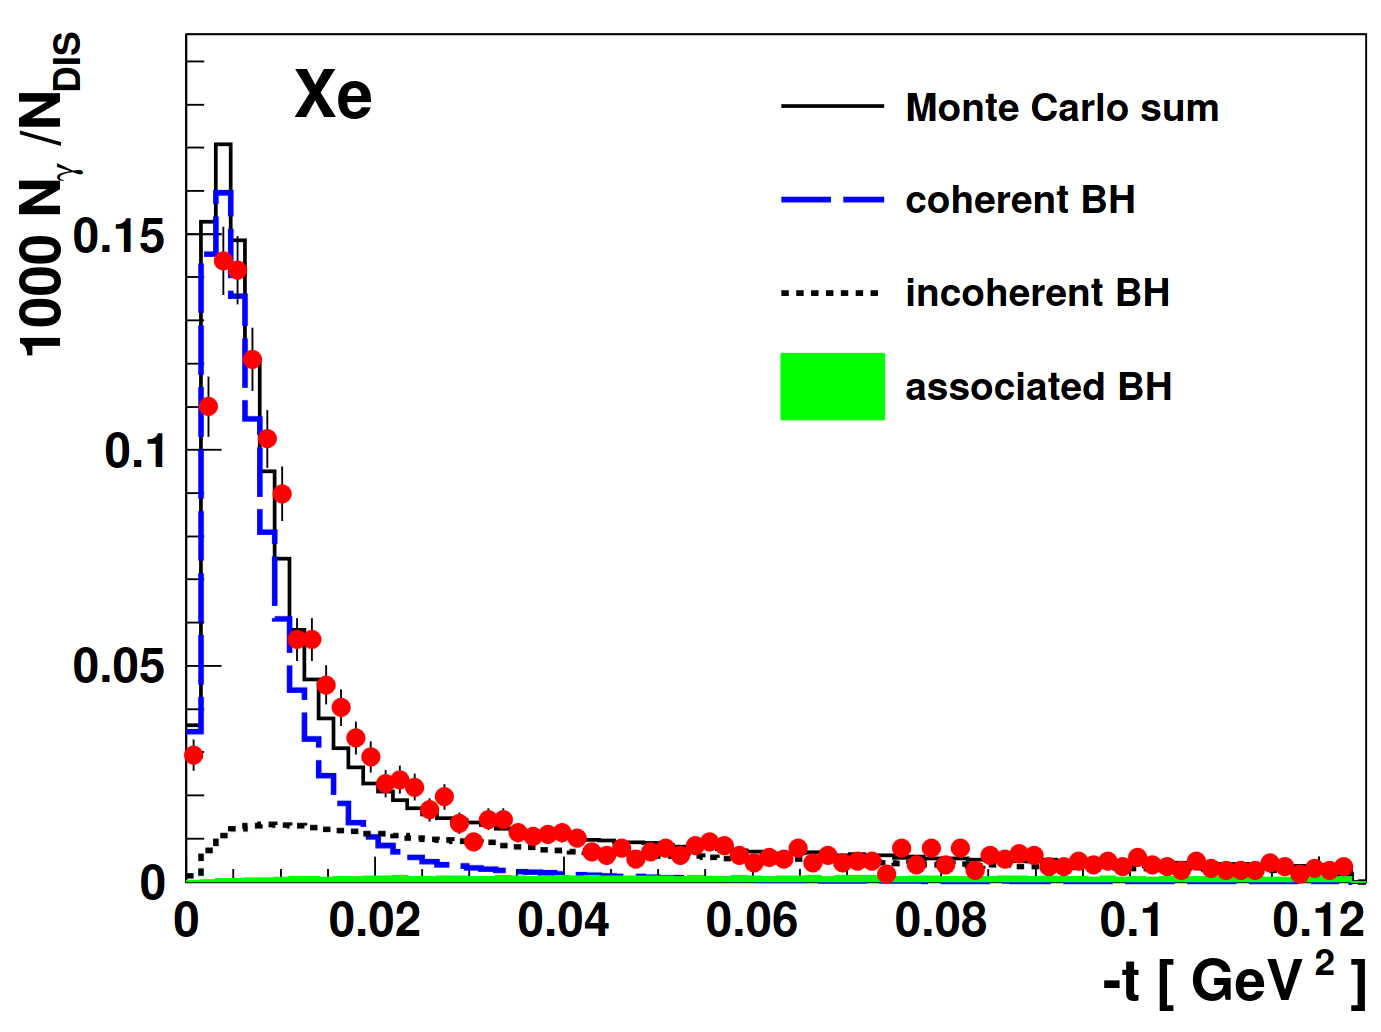
\includegraphics[width=0.9\linewidth]{figures/hermes_t_based_selection_cuts.png}
    \end{minipage}

    %\vspace{0.2cm}
    \centering
    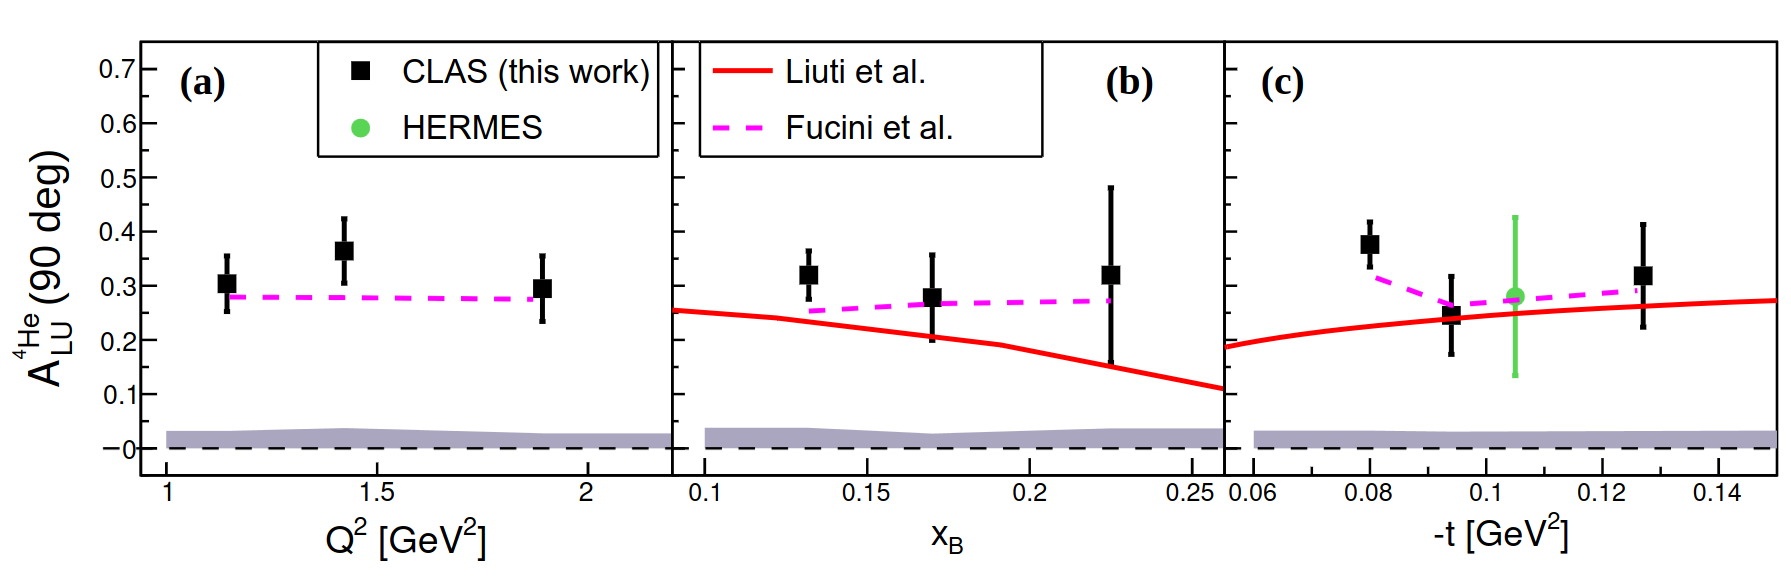
\includegraphics[width=0.63\linewidth]{figures/coherent_dvcs_bsa.png}

\end{frame}


\begin{frame}{ALERT experiment}
    \begin{itemize}
        \item ALERT is an extension of the CLAS eg6 at higher luminosity and 12 GeV
        \item It based on a new detector, A Low Energy Recoil Tracker
            \begin{itemize}
                \item Along with the $^4\mbox{He}$, identify the two isobars $^3\mbox{He}$ et $^3\mbox{H}$
                \item With kinematics: $70 < p < 400$ MeV/c, $\theta > 45^\circ$
                \item To be placed inside a 5T solenoid magnet
                \item To be transparent to the particles detected by CLAS
            \end{itemize}
        \item ALERT is a combination of a drift chamber (AHDC) and an array of scintillators (ATOF)
        % \item The design makes ALERT fast : luminosity
        % \item Identify the differents isotopes : H3, He3
    \end{itemize}

    \vspace{0.3cm}
    \centering
    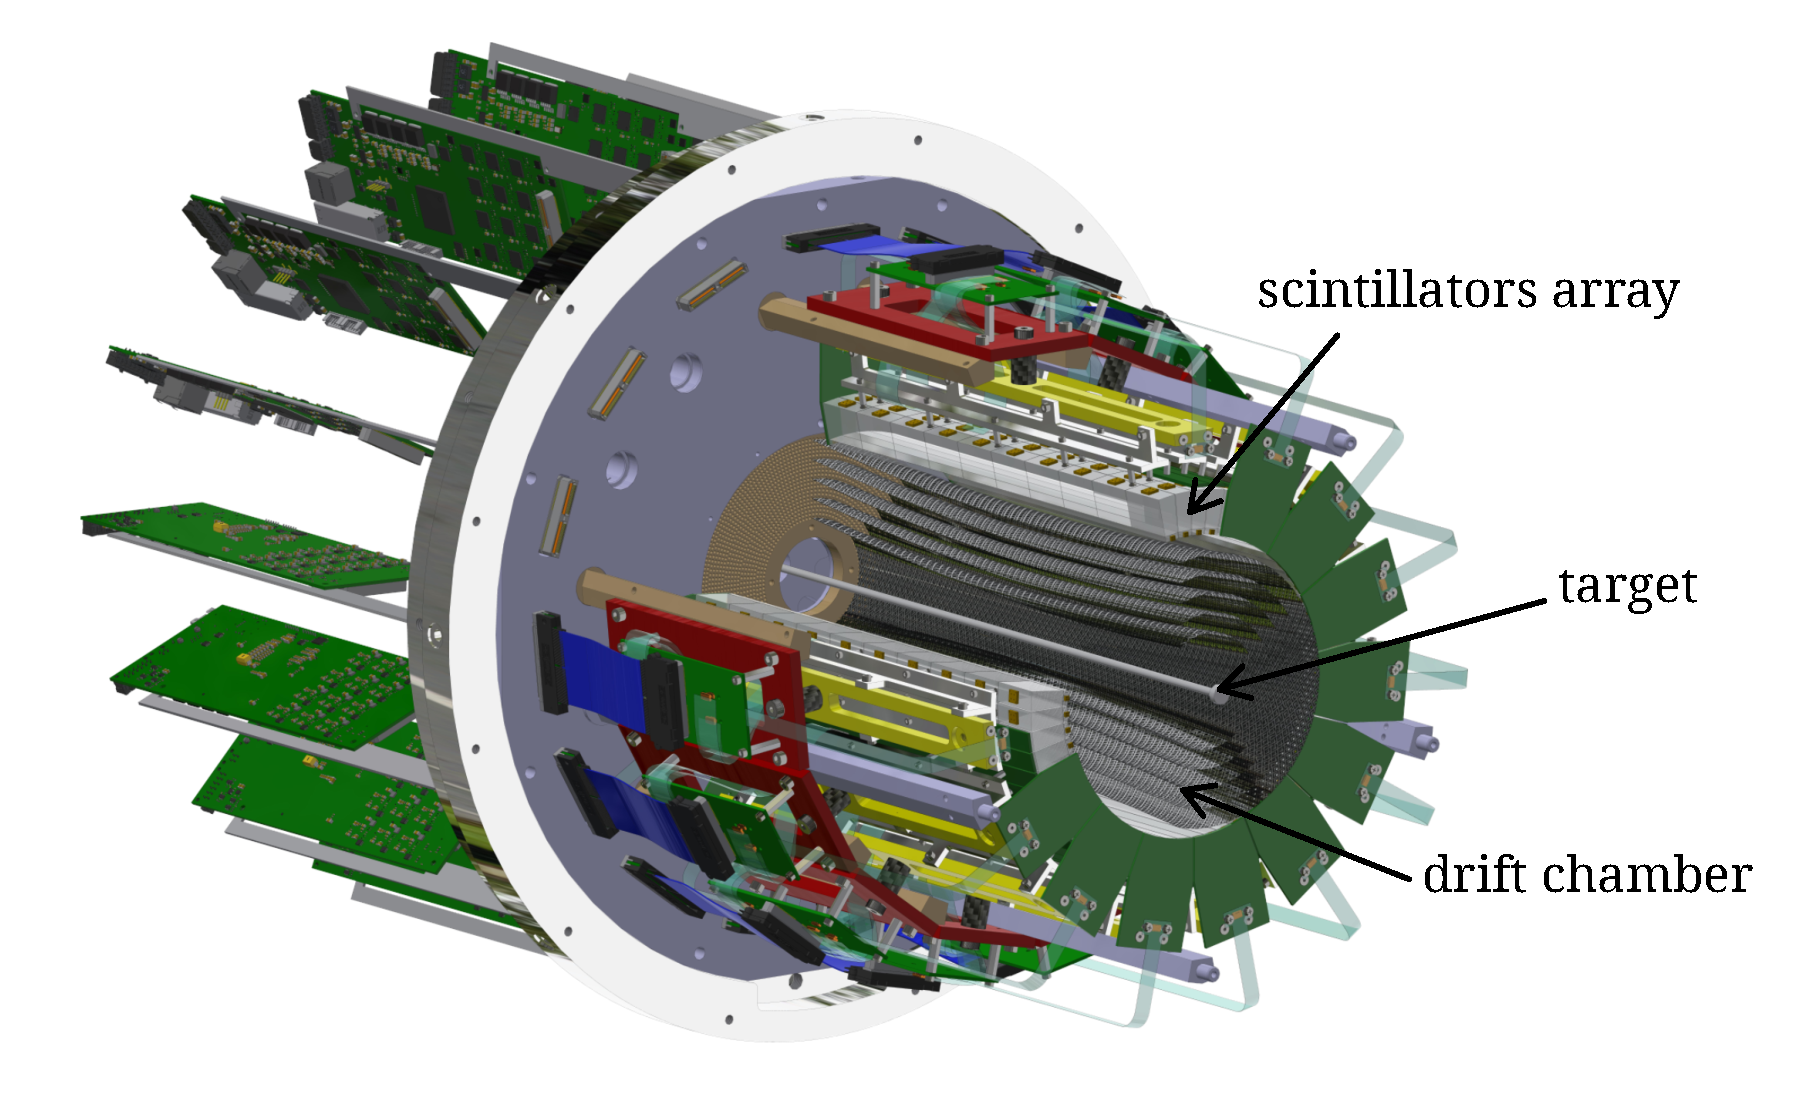
\includegraphics[width=0.45\linewidth]{figures/alert_design_annotated.pdf}
    \hspace{0.3cm}
    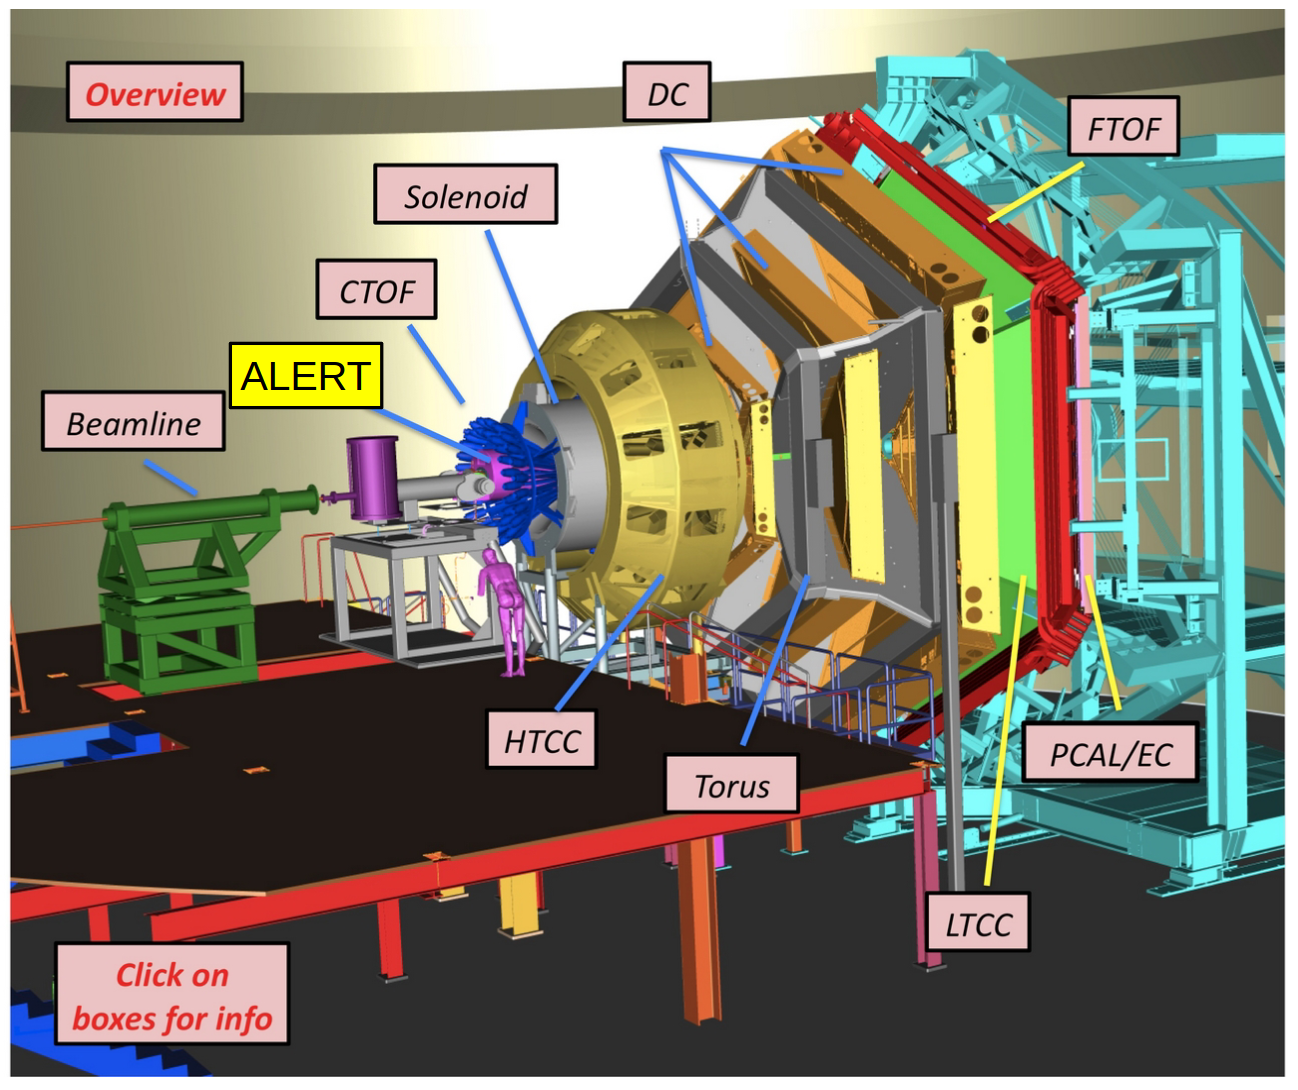
\includegraphics[width=0.38\linewidth]{figures/clas12-with-alert.png}
    
\end{frame}


\begin{frame}{ALERT run period}
    \begin{itemize}
        \item The run period took place from April 2025 to September 2025 at JLab
        \vspace{0.3cm}
        \item Run summary
            \begin{itemize}
                \item Targets: helium, deuterium, hydrogen
                \item Beam energies: 2.2 GeV, 6.4 GeV, 10.6 GeV
                \item Beam current: up to 325 nA
                \item Event rate: 10 kHz
                \item $6.42 \times 10^{10}$ trigger events collected
            \end{itemize}
        
    \end{itemize}

    \vspace{0.3cm}
    \centering
    
    \begin{minipage}[t]{0.38\textwidth}
        \vspace{0pt}
        \begin{itemize}
            \item My activities at JLab
                \begin{itemize}
                    \item Data monitoring
                    \item On-call detector expert
                    \item Target change
                    \item Target purge
                \end{itemize}
            \vspace{0.2cm}
            \item The data taking was a success
        \end{itemize}
        
    \end{minipage}
    \begin{minipage}[t]{0.6\textwidth}
        \vspace{0pt}
        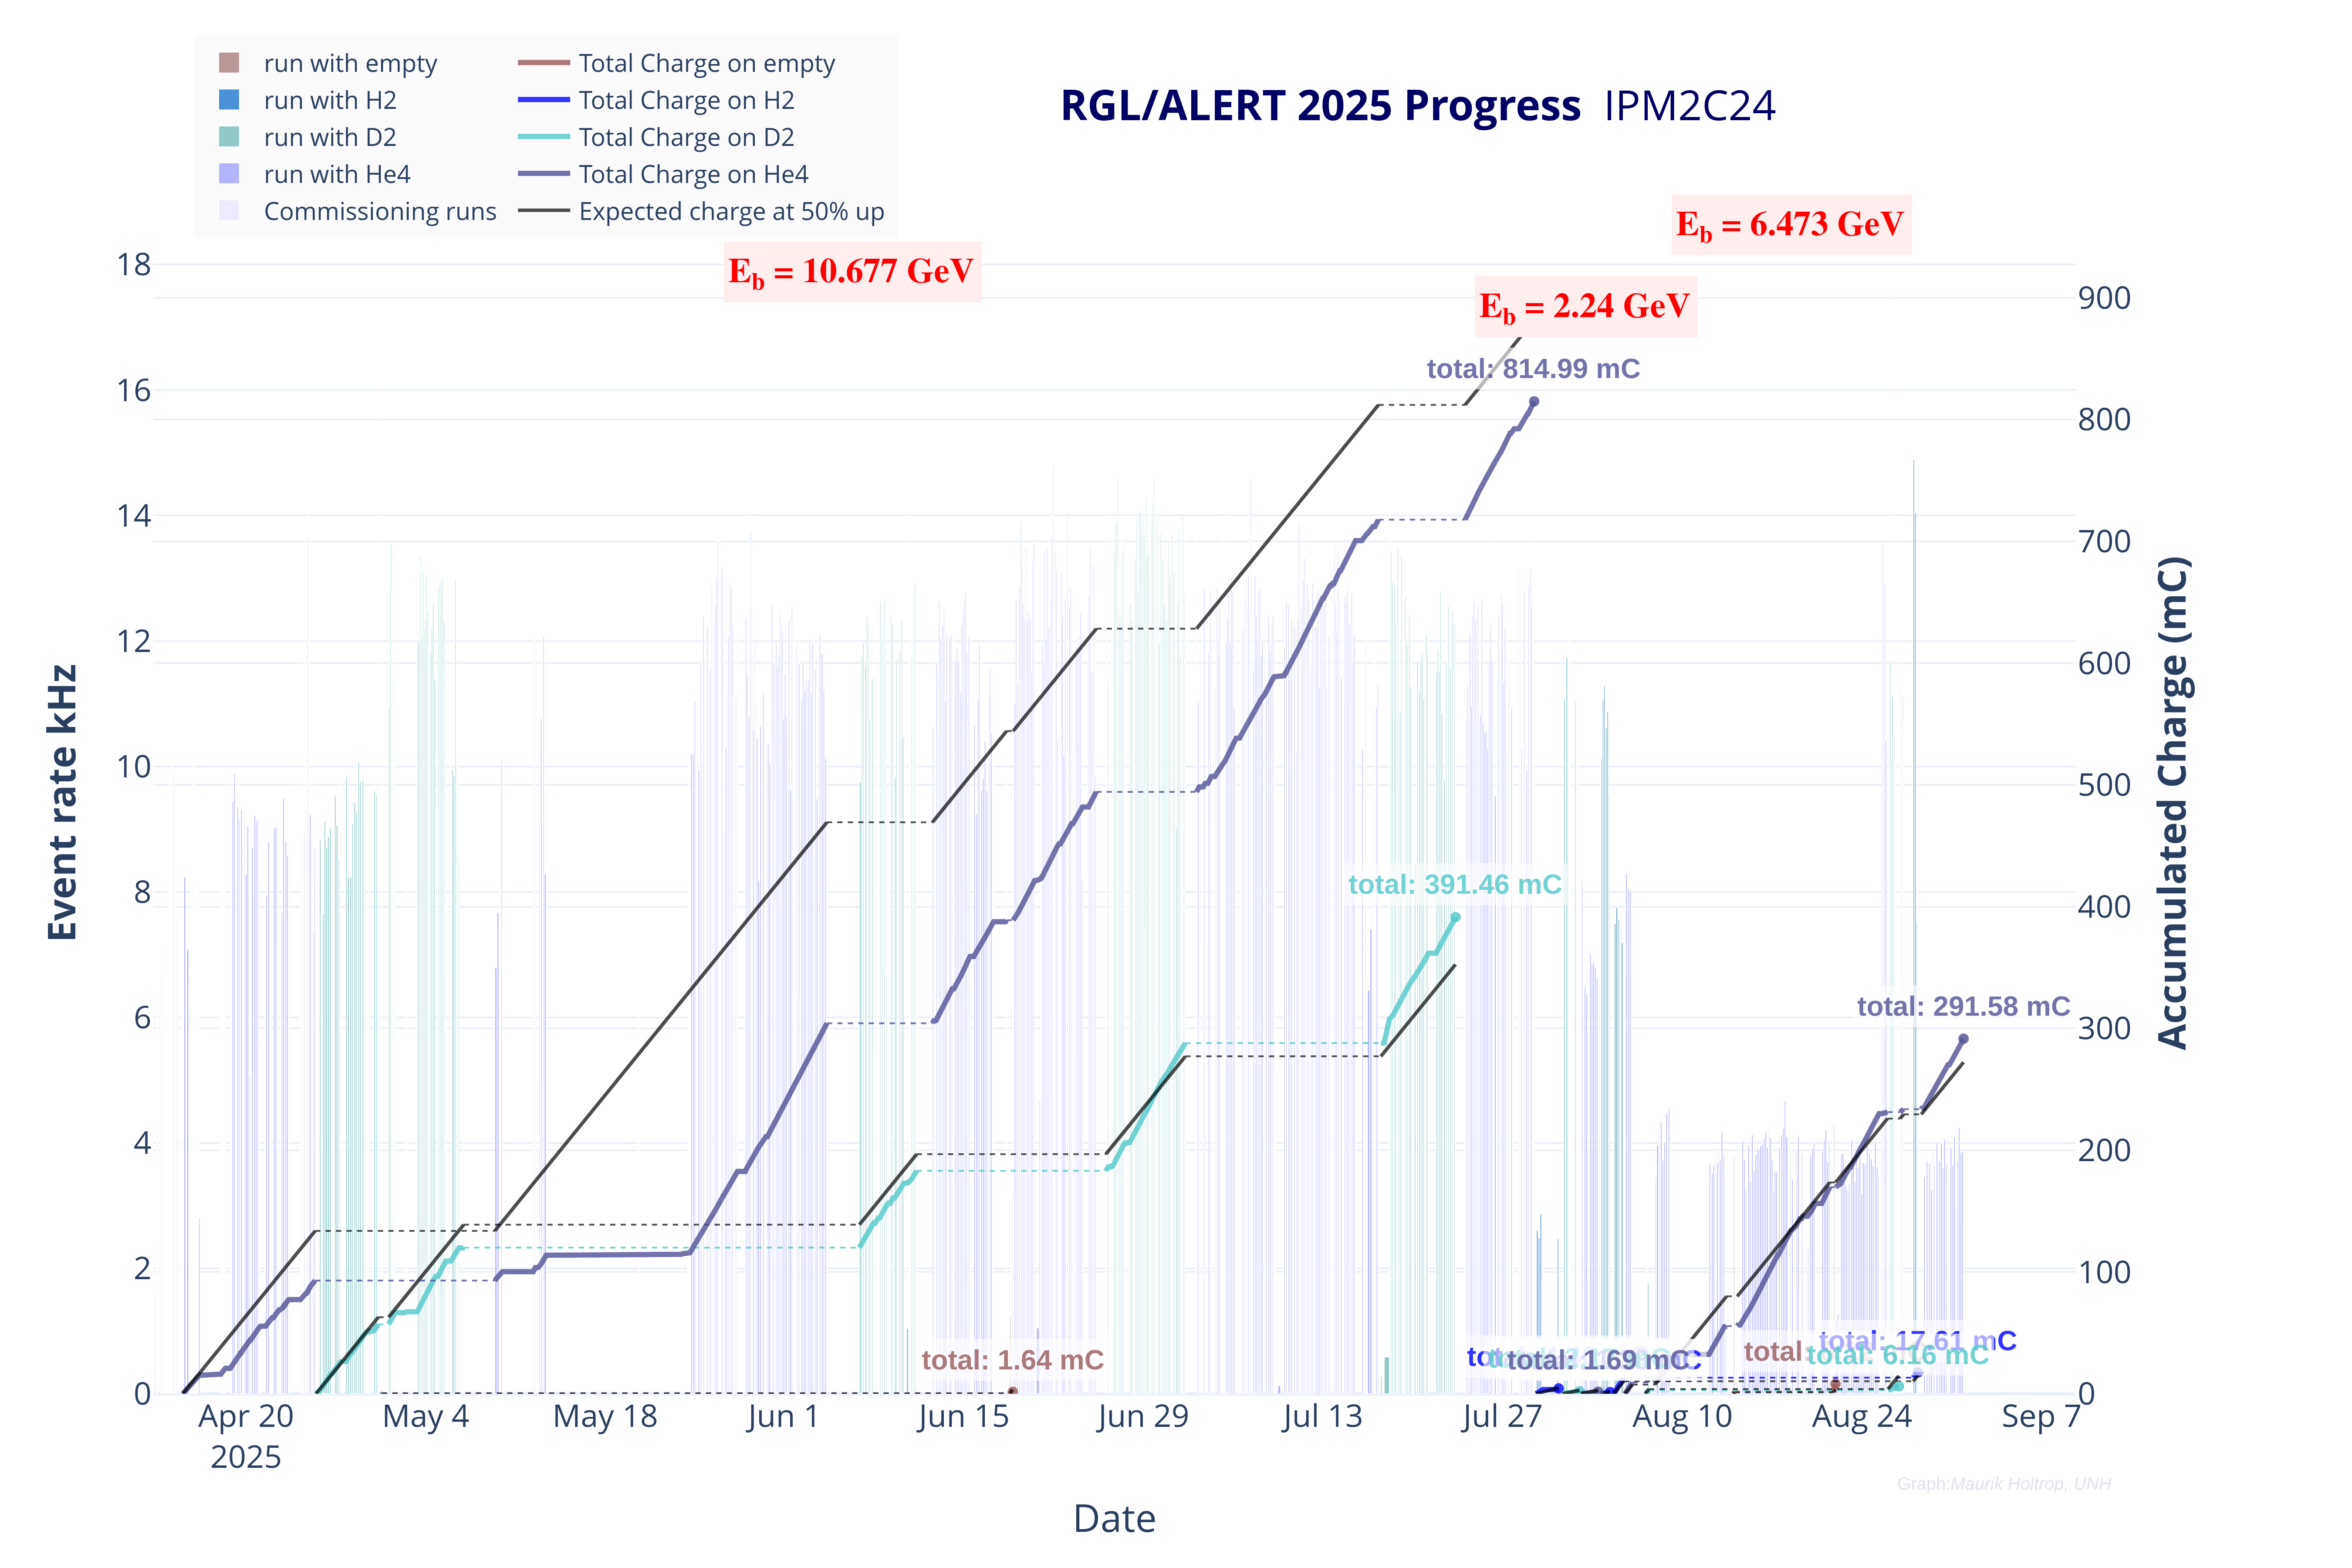
\includegraphics[width=\linewidth]{figures/HighResolutionBeamAccumulatedChargeRatio1.5.png}
    \end{minipage}
    
\end{frame}

\begin{frame}{Phase space}

    \begin{itemize}
        \item 
    \end{itemize}
    
    % 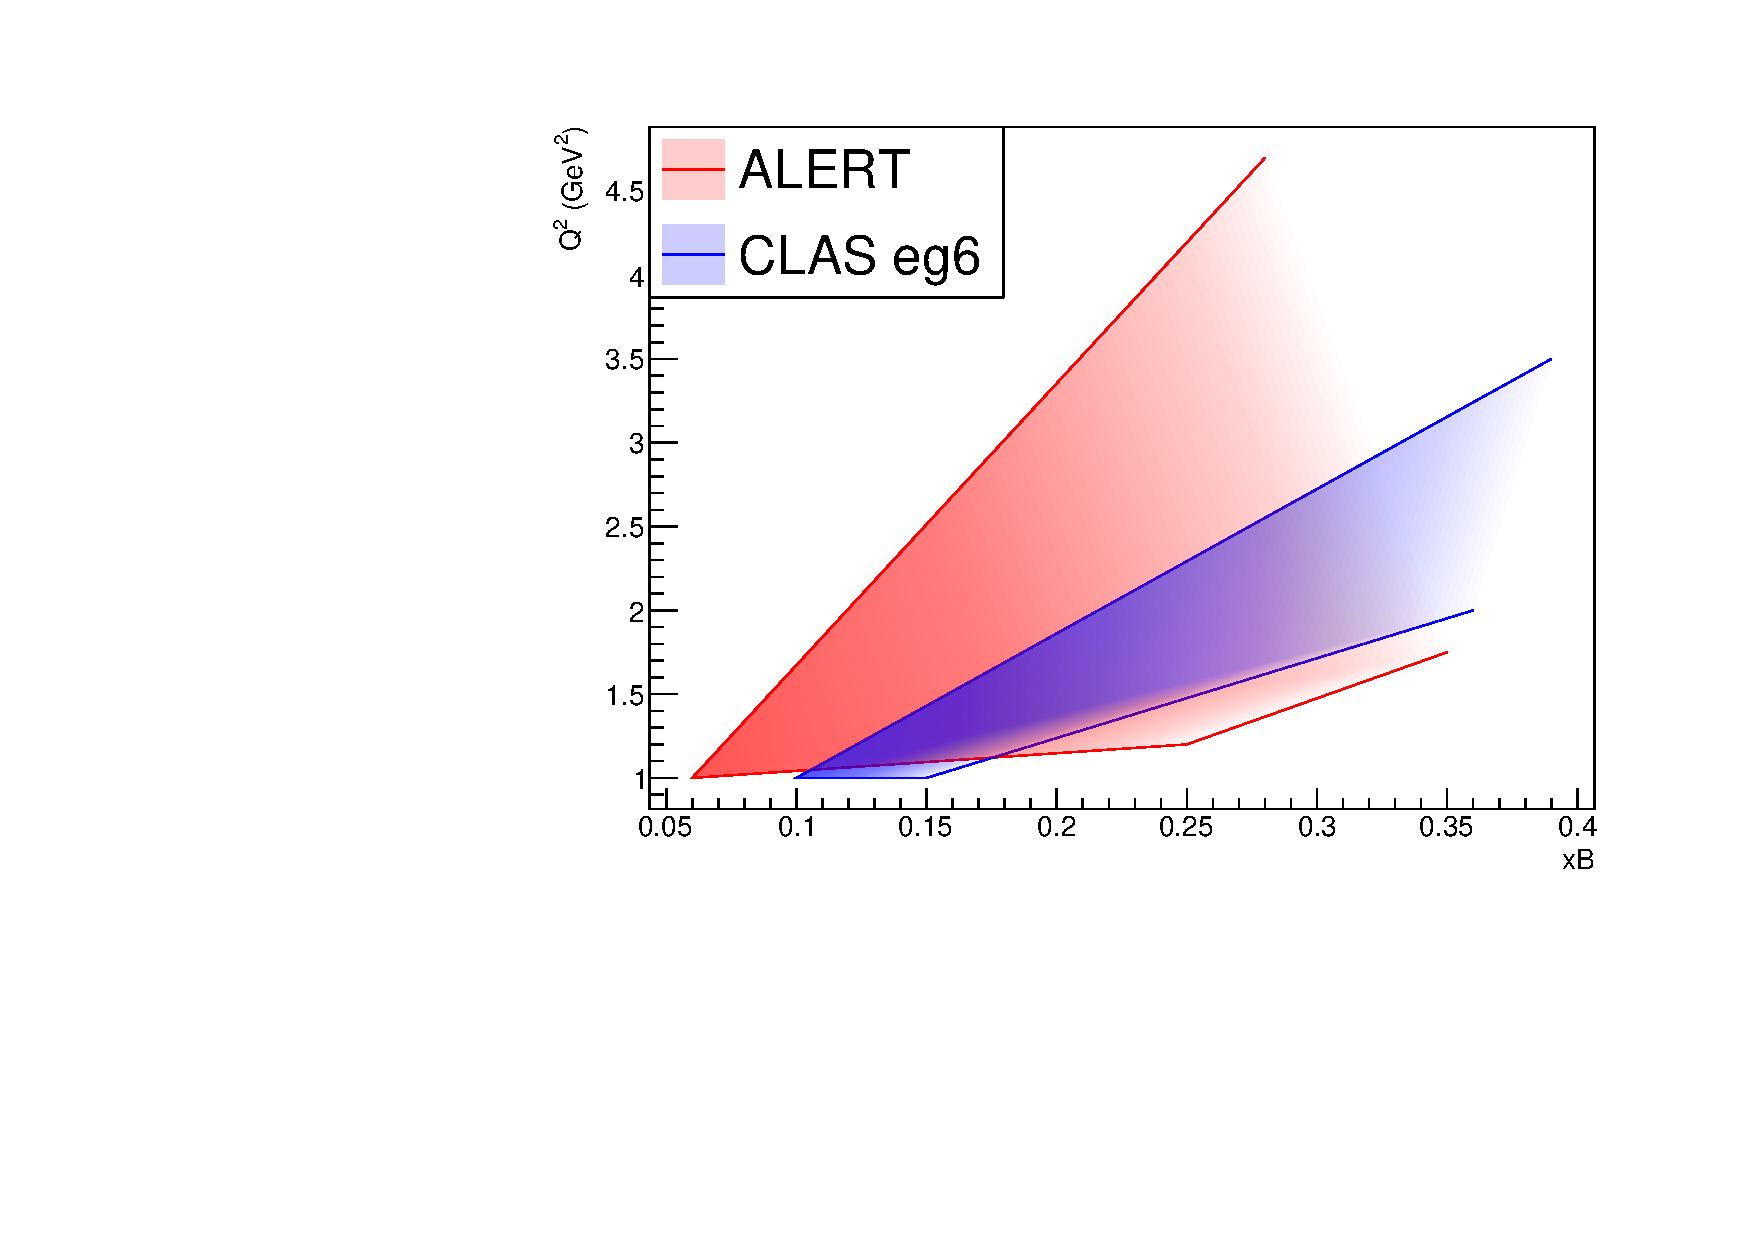
\includegraphics[width=0.3\linewidth]{figures/phase_space.pdf}

    \centering

    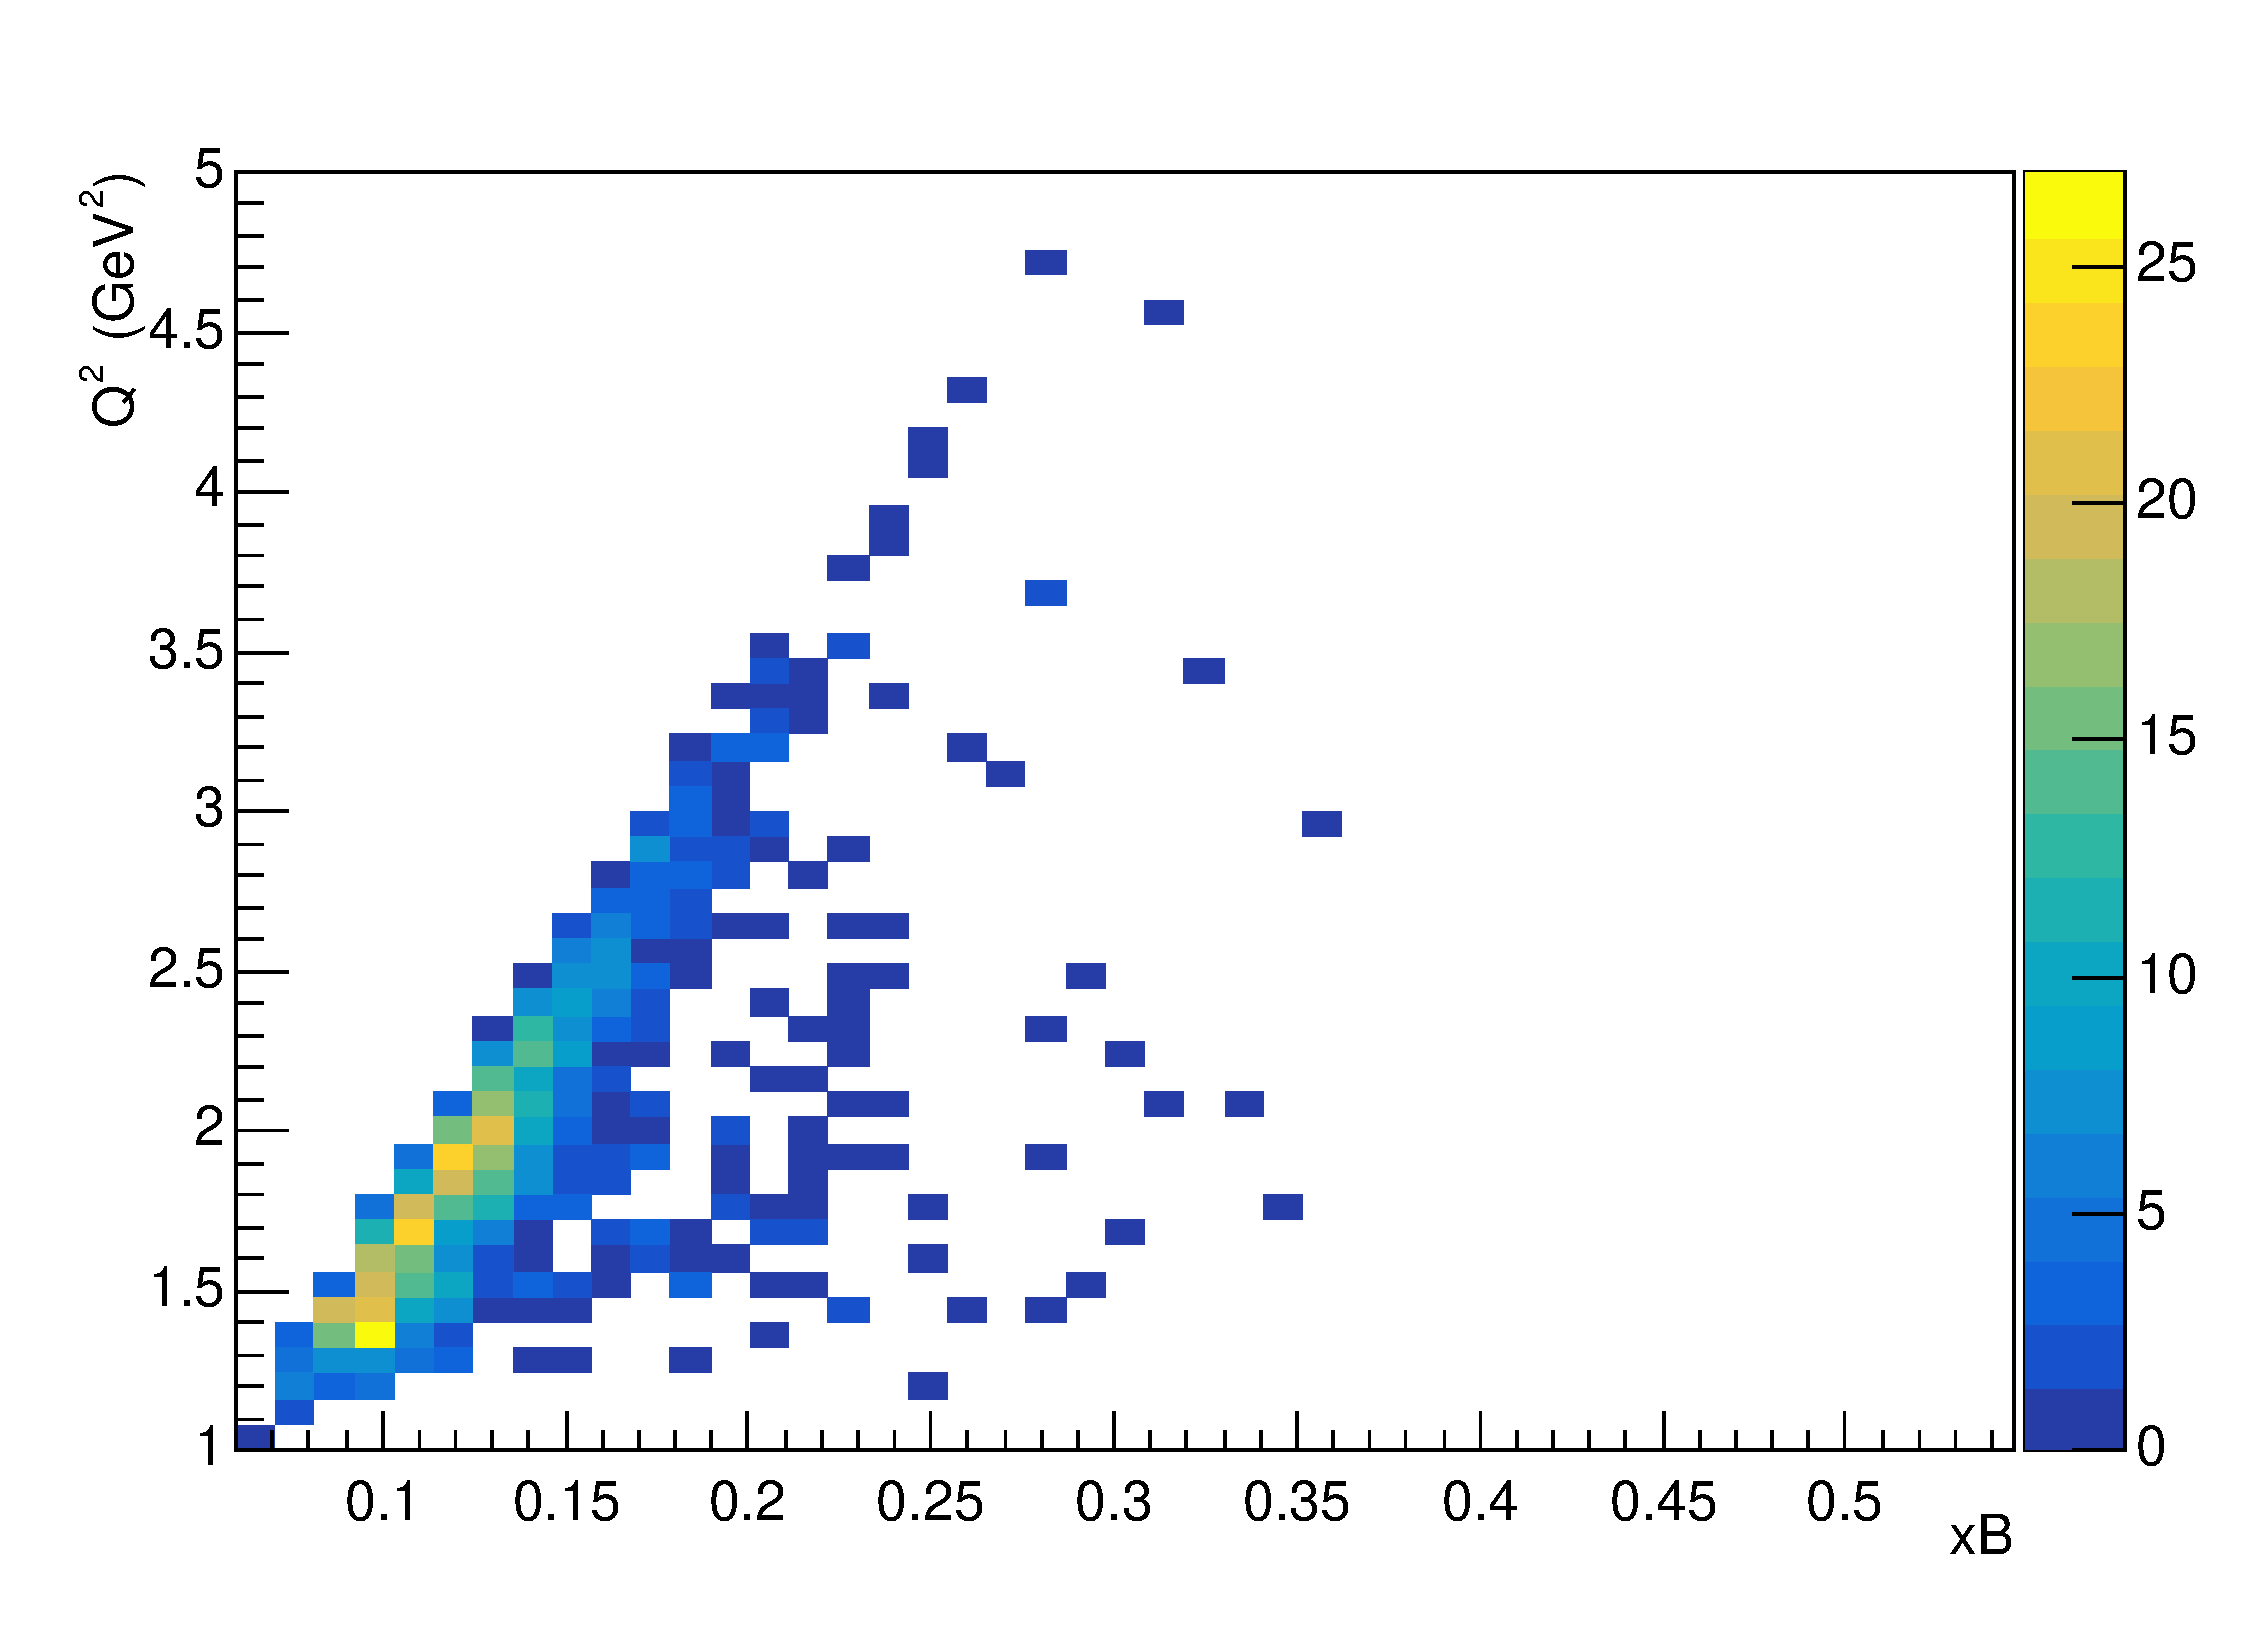
\includegraphics[width=0.4\linewidth]{figures/alert_dvcs_Q2_vs_xB.pdf}
    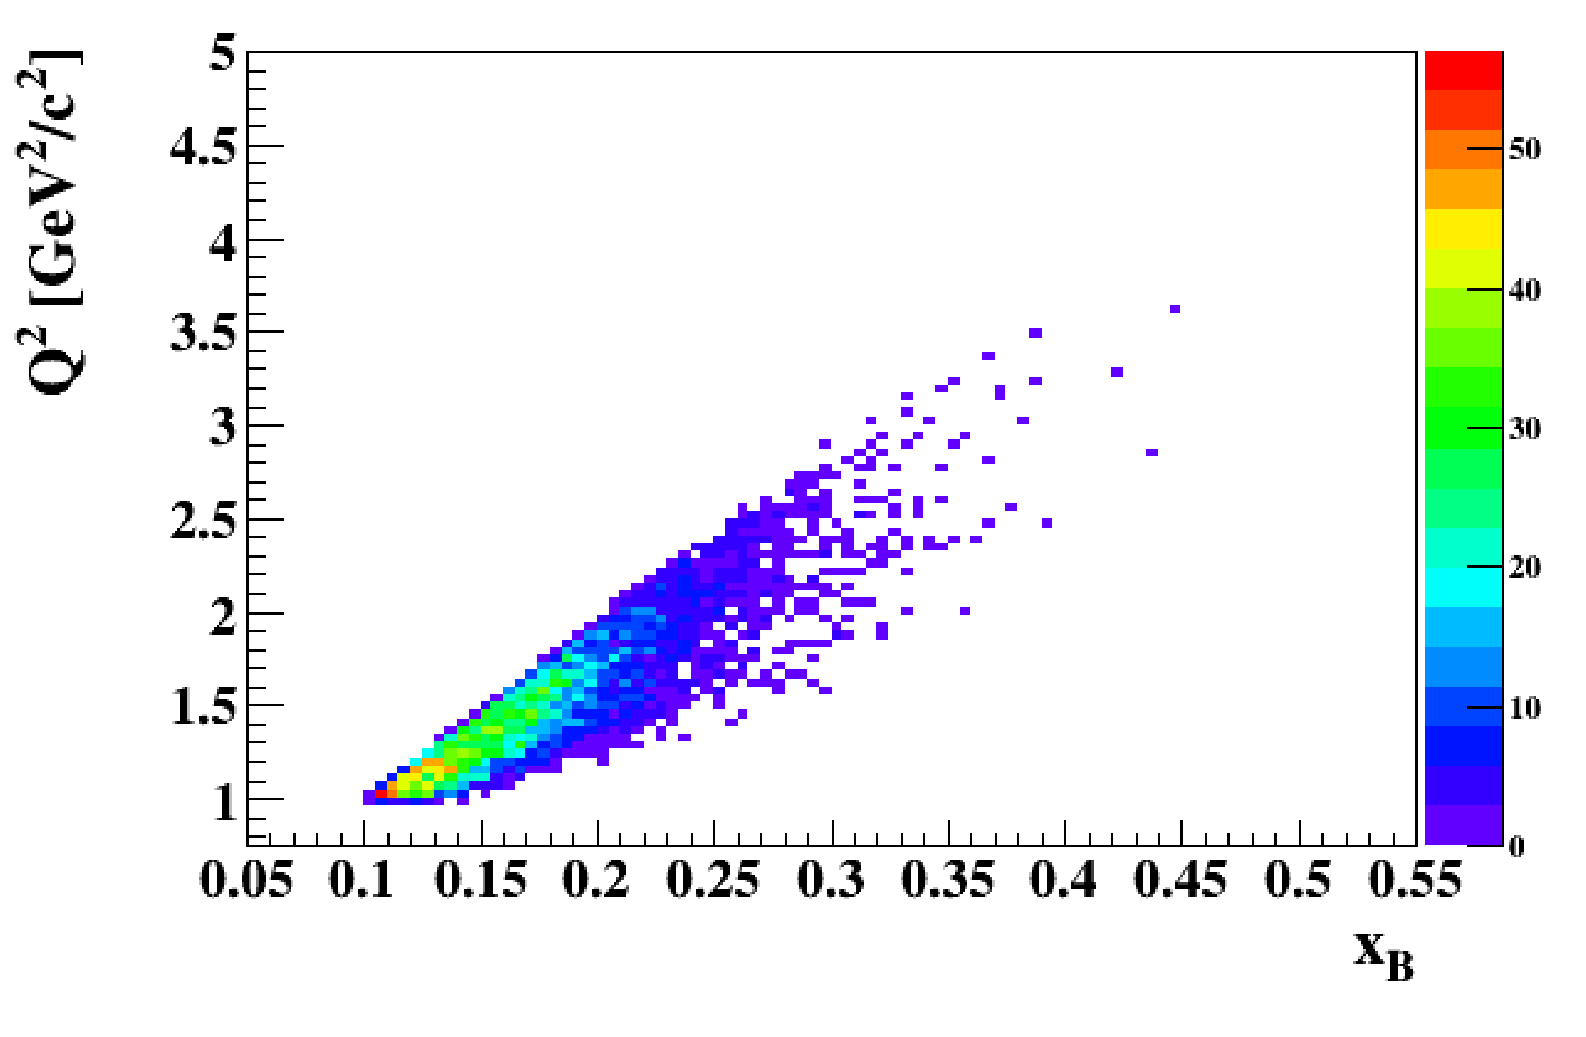
\includegraphics[width=0.4\linewidth]{figures/eg6_dvcs_Q2_vs_xB.png}
    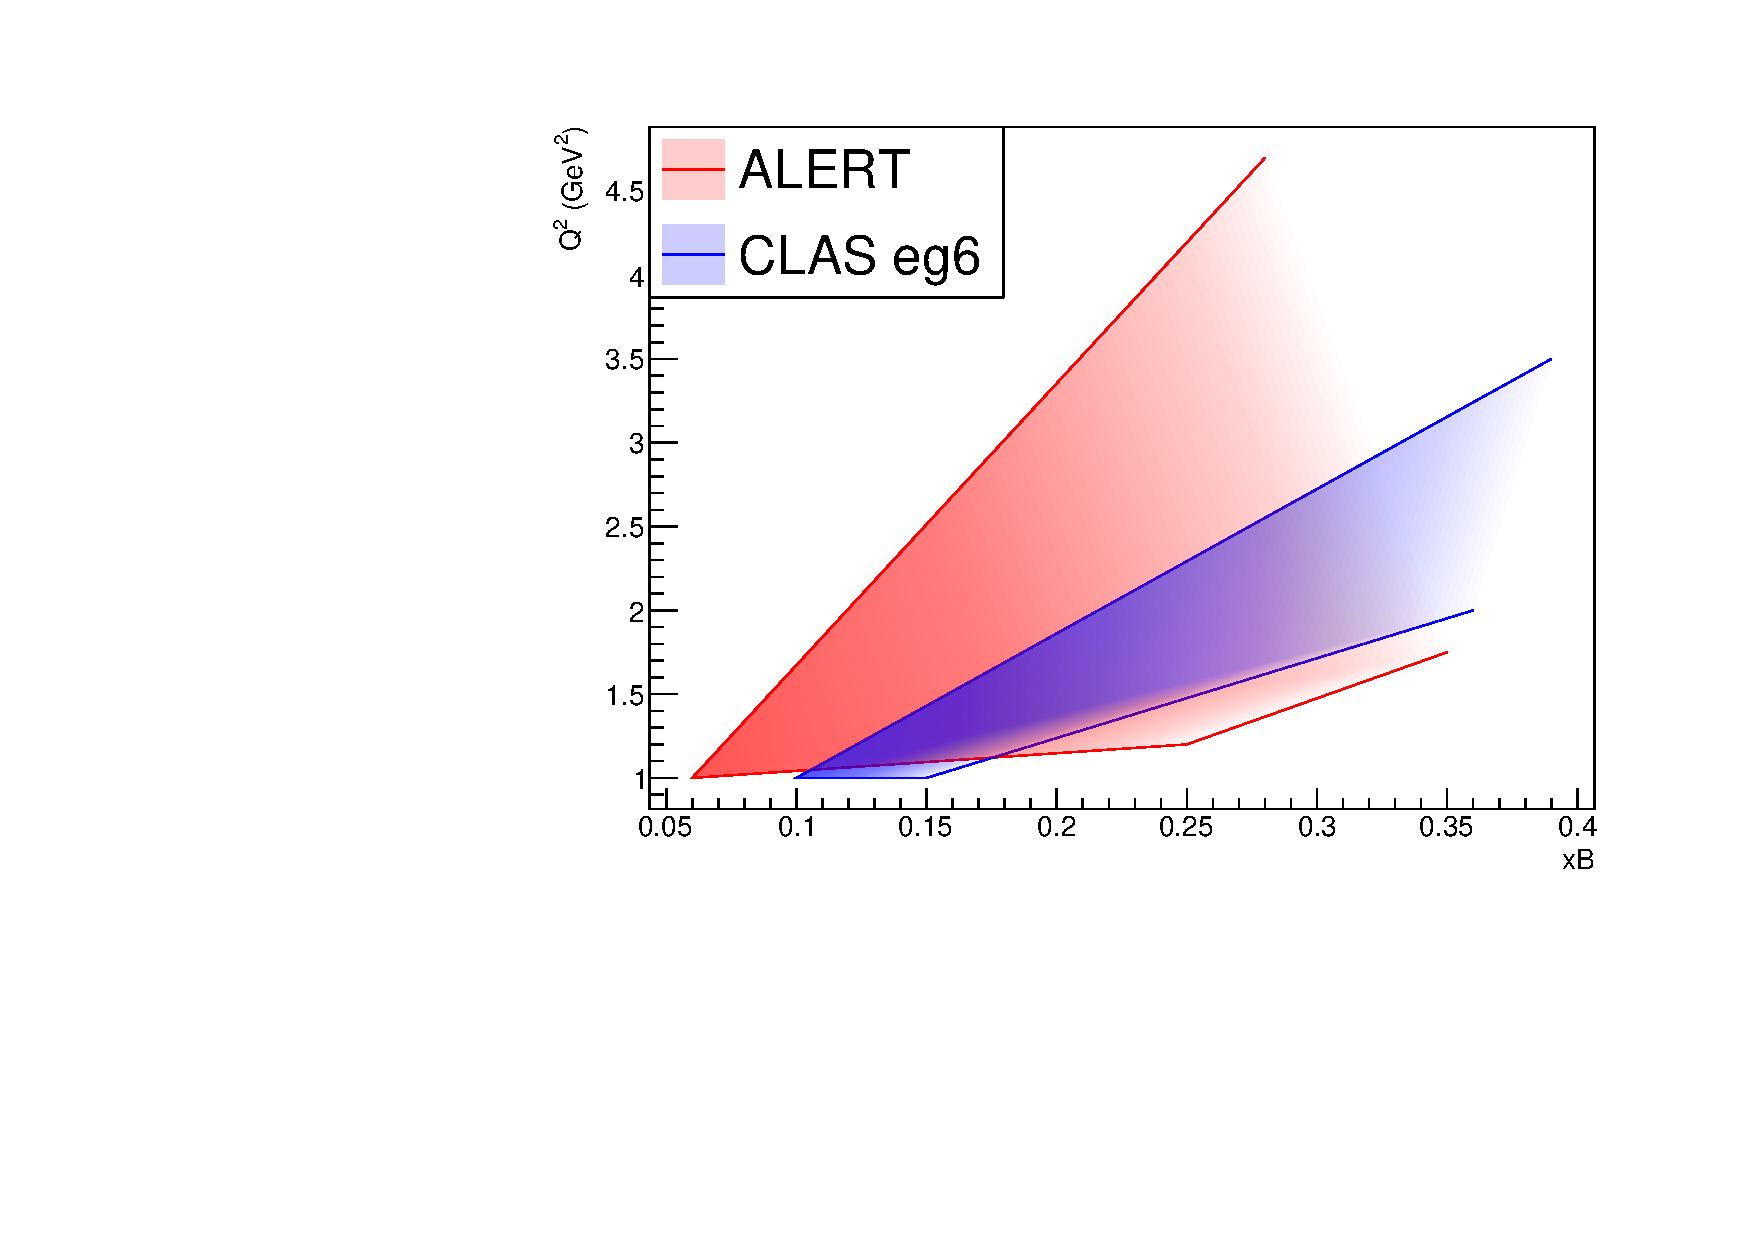
\includegraphics[width=0.4\linewidth]{figures/phase_space.pdf}
    
\end{frame}


\begin{frame}{Preliminary Beam Spin Asymmetry}

    \begin{itemize}
        \item All the work on the software and calibration is to prepare for my analysis
        \item Warnings
            \begin{itemize}
                \item The AHDC reconstruction is not completed
                \item The calibration is still ongoing (ALERT and CLAS)
                \item We made basic selection cuts
                \item The BSA has been integrated over $Q^2$, $x_{B}$ and $-t$
                \item The errors are only statistical (no $\pi ^0$ background subtraction)
                \item The study has been done on 7.53 \% of the dataset
            \end{itemize}
        \item However, we can already see an asymmetry
    \end{itemize}
    

    \centering
    %\vspace{0.2cm}

    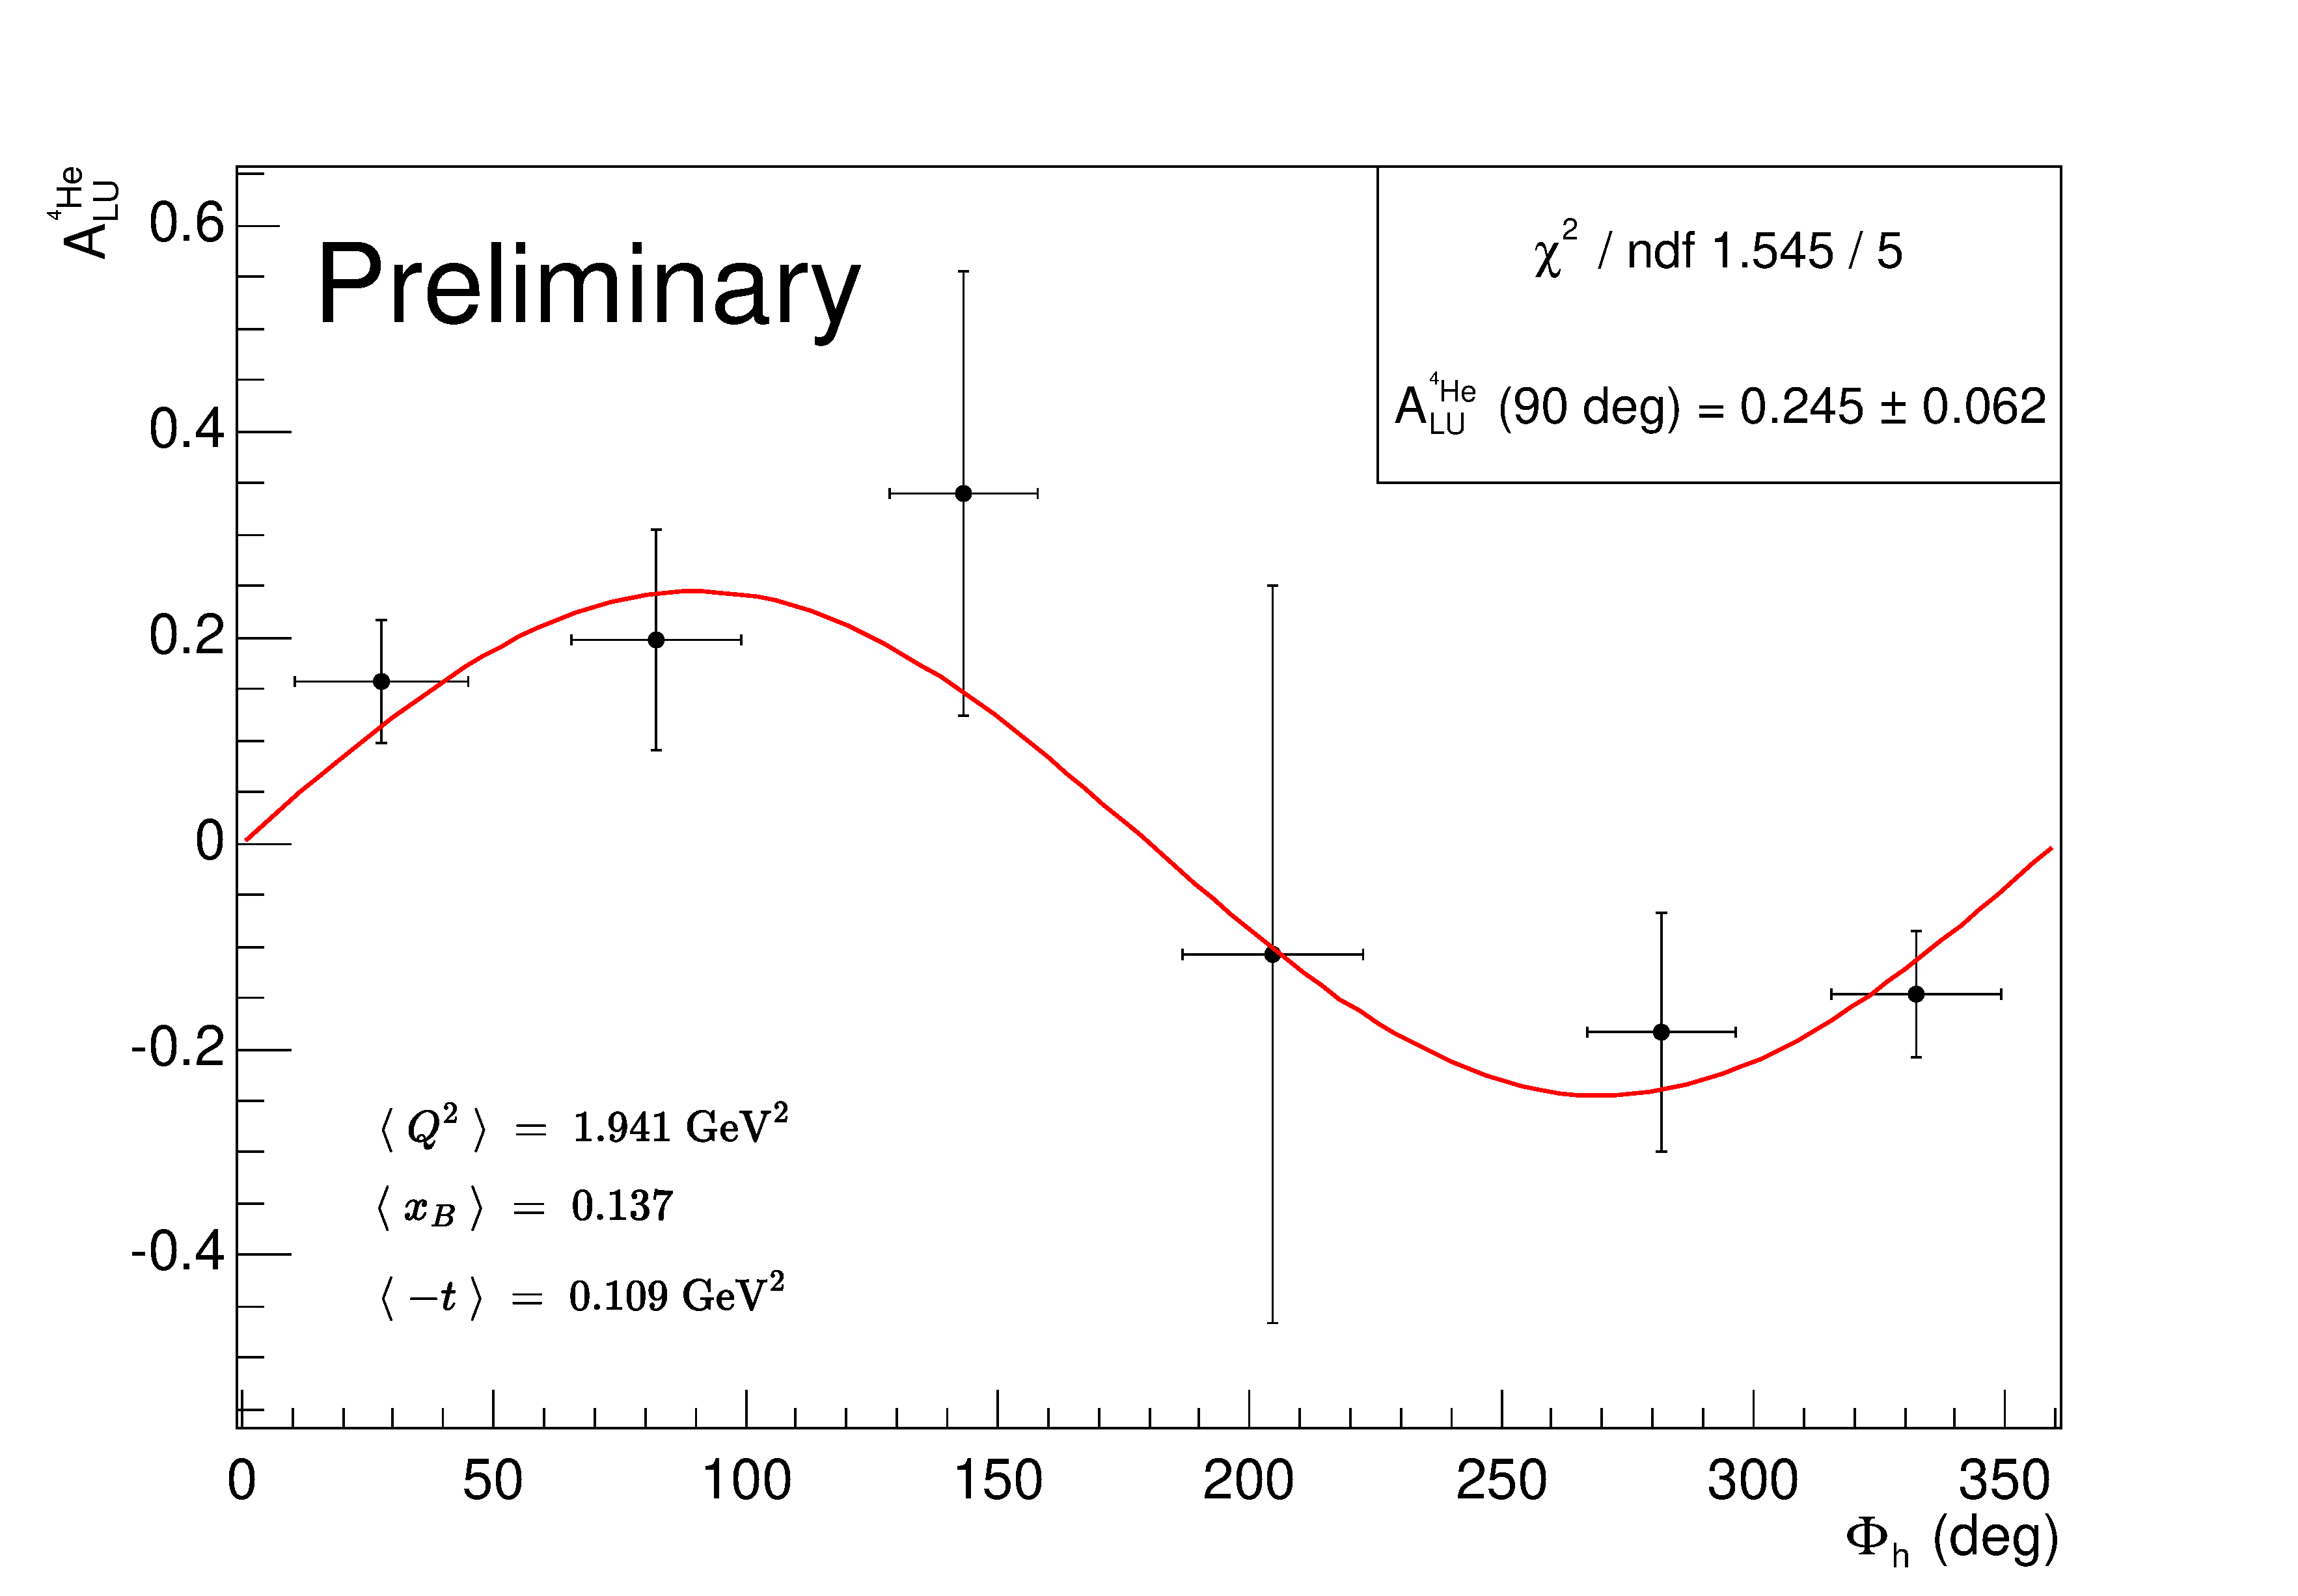
\includegraphics[width=0.5\linewidth]{figures/bsa.pdf}
    
\end{frame}










\end{document}


